\documentclass[landscape,final,a0paper,fontscale=0.285]{baposter}

\usepackage{calc}
\usepackage{graphicx}
\usepackage{epstopdf}
\usepackage{amsmath}
\usepackage{amssymb}
\usepackage{relsize}
\usepackage{multirow}
\usepackage{rotating}
\usepackage{bm}
\usepackage{url} 
\usepackage{hyperref} 

\usepackage{multicol}

%\usepackage{times}
%\usepackage{helvet}
%\usepackage{bookman}
\usepackage{palatino}

\newcommand{\captionfont}{\footnotesize}

\graphicspath{{images/}{../images/}{fig/}}
\usetikzlibrary{calc}

\newcommand{\SET}[1]  {\ensuremath{\mathcal{#1}}}
\newcommand{\MAT}[1]  {\ensuremath{\boldsymbol{#1}}}
\newcommand{\VEC}[1]  {\ensuremath{\boldsymbol{#1}}}
\newcommand{\Video}{\SET{V}}
\newcommand{\video}{\VEC{f}}
\newcommand{\track}{x}
\newcommand{\Track}{\SET T}
\newcommand{\LMs}{\SET L}
\newcommand{\lm}{l}
\newcommand{\PosE}{\SET P}
\newcommand{\posE}{\VEC p}
\newcommand{\negE}{\VEC n}
\newcommand{\NegE}{\SET N}
\newcommand{\Occluded}{\SET O}
\newcommand{\occluded}{o}

%%%%%%%%%%%%%%%%%%%%%%%%%%%%%%%%%%%%%%%%%%%%%%%%%%%%%%%%%%%%%%%%%%%%%%%%%%%%%%%%
%%%% Some math symbols used in the text
%%%%%%%%%%%%%%%%%%%%%%%%%%%%%%%%%%%%%%%%%%%%%%%%%%%%%%%%%%%%%%%%%%%%%%%%%%%%%%%%

%%%%%%%%%%%%%%%%%%%%%%%%%%%%%%%%%%%%%%%%%%%%%%%%%%%%%%%%%%%%%%%%%%%%%%%%%%%%%%%%
% Multicol Settings
%%%%%%%%%%%%%%%%%%%%%%%%%%%%%%%%%%%%%%%%%%%%%%%%%%%%%%%%%%%%%%%%%%%%%%%%%%%%%%%%
\setlength{\columnsep}{1.5em}
\setlength{\columnseprule}{0mm}

%%%%%%%%%%%%%%%%%%%%%%%%%%%%%%%%%%%%%%%%%%%%%%%%%%%%%%%%%%%%%%%%%%%%%%%%%%%%%%%%
% Save space in lists. Use this after the opening of the list
%%%%%%%%%%%%%%%%%%%%%%%%%%%%%%%%%%%%%%%%%%%%%%%%%%%%%%%%%%%%%%%%%%%%%%%%%%%%%%%%
\newcommand{\compresslist}{%
\setlength{\itemsep}{1pt}%
\setlength{\parskip}{0pt}%
\setlength{\parsep}{0pt}%
}

%%%%%%%%%%%%%%%%%%%%%%%%%%%%%%%%%%%%%%%%%%%%%%%%%%%%%%%%%%%%%%%%%%%%%%%%%%%%%%
%%% Begin of Document
%%%%%%%%%%%%%%%%%%%%%%%%%%%%%%%%%%%%%%%%%%%%%%%%%%%%%%%%%%%%%%%%%%%%%%%%%%%%%%

\begin{document}

%%%%%%%%%%%%%%%%%%%%%%%%%%%%%%%%%%%%%%%%%%%%%%%%%%%%%%%%%%%%%%%%%%%%%%%%%%%%%%
%%% Here starts the poster
%%%---------------------------------------------------------------------------
%%% Format it to your taste with the options
%%%%%%%%%%%%%%%%%%%%%%%%%%%%%%%%%%%%%%%%%%%%%%%%%%%%%%%%%%%%%%%%%%%%%%%%%%%%%%
% Define some colors

%\definecolor{lightblue}{cmyk}{0.83,0.24,0,0.12}
\definecolor{lightblue}{rgb}{0.145,0.6666,1}

% Draw a video
\newlength{\FSZ}
\newcommand{\drawvideo}[3]{% [0 0.25 0.5 0.75 1 1.25 1.5]
   \noindent\pgfmathsetlength{\FSZ}{\linewidth/#2}
   \begin{tikzpicture}[outer sep=0pt,inner sep=0pt,x=\FSZ,y=\FSZ]
   \draw[color=lightblue!50!black] (0,0) node[outer sep=0pt,inner sep=0pt,text width=\linewidth,minimum height=0] (video) {\noindent#3};
   \path [fill=lightblue!50!black,line width=0pt] 
     (video.north west) rectangle ([yshift=\FSZ] video.north east) 
    \foreach \x in {1,2,...,#2} {
      {[rounded corners=0.6] ($(video.north west)+(-0.7,0.8)+(\x,0)$) rectangle +(0.4,-0.6)}
    }
;
   \path [fill=lightblue!50!black,line width=0pt] 
     ([yshift=-1\FSZ] video.south west) rectangle (video.south east) 
    \foreach \x in {1,2,...,#2} {
      {[rounded corners=0.6] ($(video.south west)+(-0.7,-0.2)+(\x,0)$) rectangle +(0.4,-0.6)}
    }
;
   \foreach \x in {1,...,#1} {
     \draw[color=lightblue!50!black] ([xshift=\x\linewidth/#1] video.north west) -- ([xshift=\x\linewidth/#1] video.south west);
   }
   \foreach \x in {0,#1} {
     \draw[color=lightblue!50!black] ([xshift=\x\linewidth/#1,yshift=1\FSZ] video.north west) -- ([xshift=\x\linewidth/#1,yshift=-1\FSZ] video.south west);
   }
   \end{tikzpicture}
}

\newcommand{\setS}{\mathbf{G}}
\newcommand{\comp}{C}
\newcommand{\TranscodeIndicator}{P}
\newcommand{\RequestingSeg}{\mathbf{K}}
\newcommand{\TranscodeSet}{\mathbf{E}}
\newcommand{\IdleComp}{I}
\newcommand{\SegRepCost}{F}
\newcommand{\Assign}{A}
\newcommand{\ReqFromRegion}{J}
\newcommand{\CDNRegions}{\mathbf{R}}
\newcommand{\Users}{\mathbf{U}}
\newcommand{\Redirect}{D}
\newcommand{\RegionRepCost}{Z}
\newcommand{\bandwidth}{W}
\newcommand{\Version}{L}
\newcommand{\USPref}{H}
\newcommand{\ReqOfSeg}{Q}
\newcommand{\SegQuality}{Y}
\newcommand{\Bitrate}{B}


\hyphenation{resolution occlusions}
%%
\begin{poster}%
  % Poster Options
  {
  % Show grid to help with alignment
  grid=false,
  % Column spacing
  colspacing=1em,
  % Color style
  bgColorOne=white,
  bgColorTwo=white,
  borderColor=lightblue,
  headerColorOne=white,%blue,
  headerColorTwo=white,%lightblue,
  headerFontColor=blue,%white,
  boxColorOne=white,
  boxColorTwo=lightblue,
  % Format of textbox
  textborder=roundedsmall,%roundedleft,
  % Format of text header
  eyecatcher=true,
  headerborder=closed,
  headerheight=0.125\textheight,
%  textfont=\sc, An example of changing the text font
  headershape=smallrounded,
  headershade=shadelr,
  headerfont=\Large\bf\textsc, %Sans Serif
  textfont={\setlength{\parindent}{1.5em}},
  boxshade=plain,
%  background=shade-tb,
  background=plain,
  linewidth=2pt
  }
  % Eye Catcher
  {
\includegraphics[height=5em]{logo/PearLogo.eps}} 
  % Title
  {\bf{A Joint Online Transcoding and Delivery Approach\\ for Dynamic Adaptive Streaming}\vspace{0.25em}}
  % Authors
  {\textsc{ Alan Zhuang      }  \href{mailto:a@pear.hk}{\nolinkurl{a@pear.hk}}}
  % University logo
  {% The makebox allows the title to flow into the logo, this is a hack because of the L shaped logo.
    
\includegraphics[height=5em]{logo/UST4C_L4.eps}
  }

%%%%%%%%%%%%%%%%%%%%%%%%%%%%%%%%%%%%%%%%%%%%%%%%%%%%%%%%%%%%%%%%%%%%%%%%%%%%%%
%%% Now define the boxes that make up the poster
%%%---------------------------------------------------------------------------
%%% Each box has a name and can be placed absolutely or relatively.
%%% The only inconvenience is that you can only specify a relative position 
%%% towards an already declared box. So if you have a box attached to the 
%%% bottom, one to the top and a third one which should be in between, you 
%%% have to specify the top and bottom boxes before you specify the middle 
%%% box.
%%%%%%%%%%%%%%%%%%%%%%%%%%%%%%%%%%%%%%%%%%%%%%%%%%%%%%%%%%%%%%%%%%%%%%%%%%%%%%
    %
    % A coloured circle useful as a bullet with an adjustably strong filling
    \newcommand{\colouredcircle}{%
      \tikz{\useasboundingbox (-0.2em,-0.32em) rectangle(0.2em,0.32em); \draw[draw=black,fill=lightblue,line width=0.03em] (0,0) circle(0.18em);}}

%%%%%%%%%%%%%%%%%%%%%%%%%%%%%%%%%%%%%%%%%%%%%%%%%%%%%%%%%%%%%%%%%%%%%%%%%%%%%%
  \headerbox{Background}{name=background,span=1,column=0,row=0}{
%%%%%%%%%%%%%%%%%%%%%%%%%%%%%%%%%%%%%%%%%%%%%%%%%%%%%%%%%%%%%%%%%%%%%%%%%%%%%%
\noindent
Popular online video sites \\
   %\begin{center}
    \drawvideo{4}{40}{%
   		
\includegraphics[height=2.7em]{logo/YouTube.eps}%
   		
\includegraphics[height=2.6em]{logo/Netflix.eps}%
   		
\includegraphics[height=2.7em]{logo/youku.png}%
   		
\includegraphics[height=2.7em]{logo/tencent_video.png}%
   	}
   %\end{center}
   transcode their vidoes to multiple versions\\
   $$\rightarrow \{ ~mp4, [H.264, AAC]~ \}\left\{
   \begin{array}{ll}
   version_1     & {(x_1 ~ kbps)}\\
   version_2     & {(x_2 ~ kbps)}\\
   \vdots     & {\vdots}\\
   version_n     & {(x_n ~ kbps)}
   \end{array} \right. $$
   and then stream them through the network, \\
   %\begin{enumerate}\compresslist
   %   \item Appearance changes due to lighting and pose
   %   \item Occlusions
   %   \item Speed: Interactive editing requires faster than framerate calculation
   %\end{enumerate}
   %\begin{center}
   	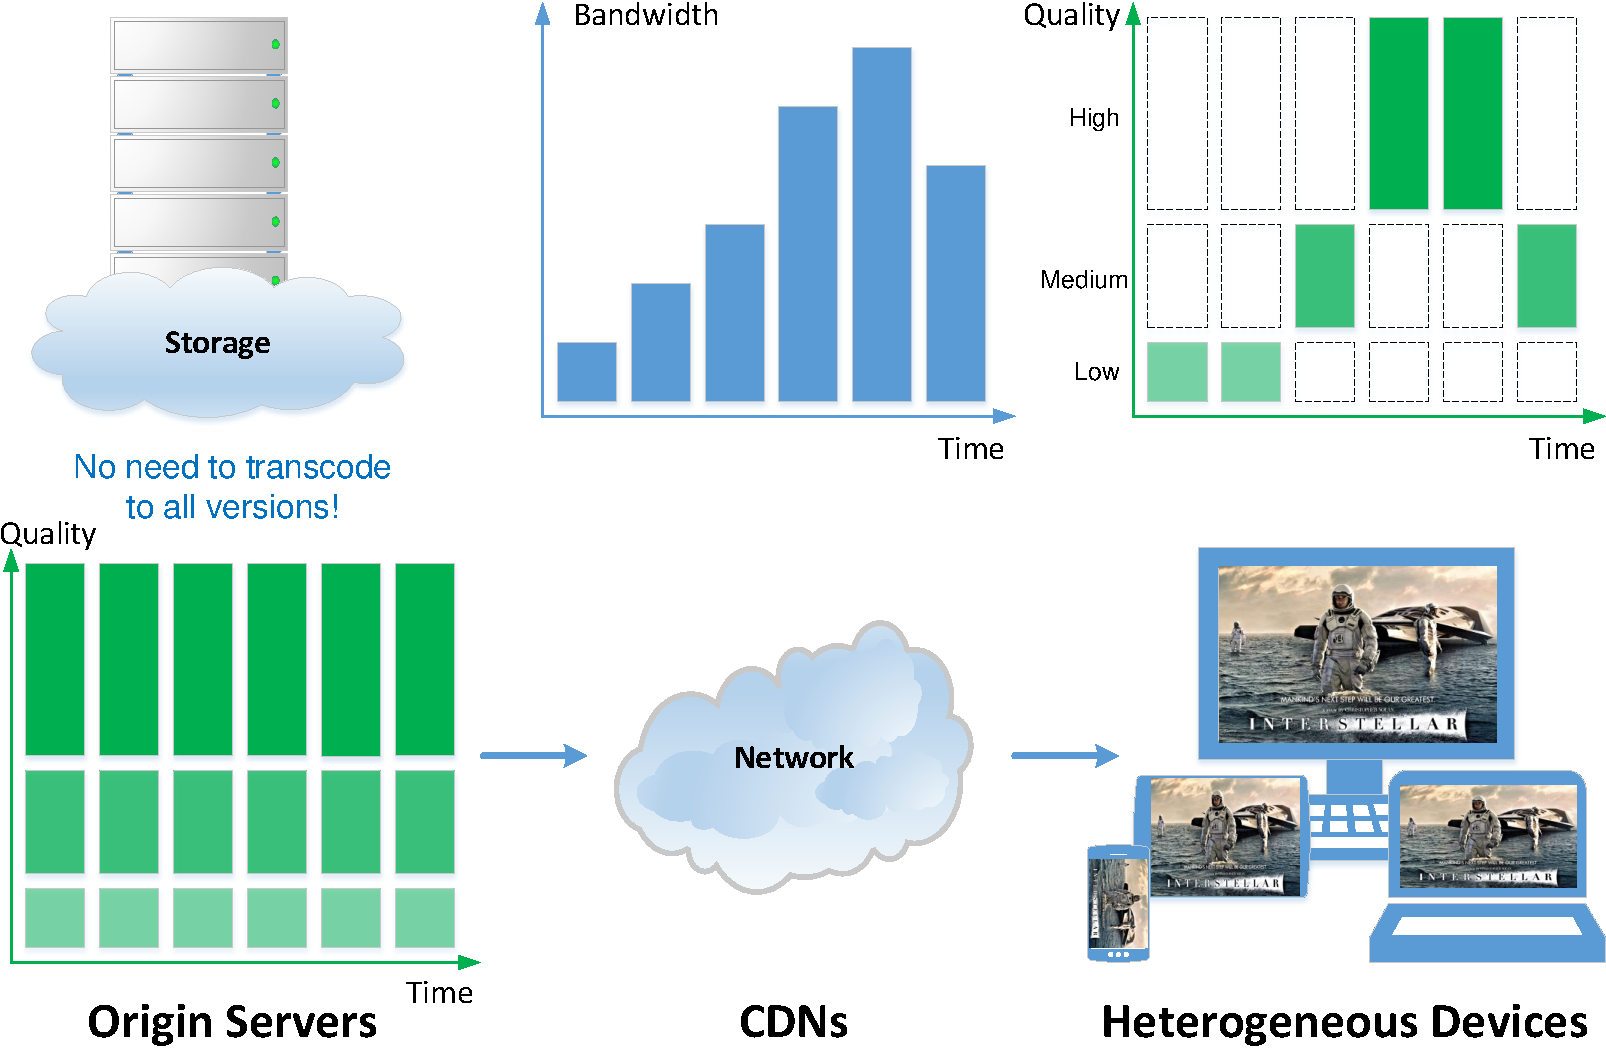
\includegraphics[width=\linewidth]{fig/adaptive_streaming_arch.pdf}
   %\end{center}
   so that users can enjoy a better watching experience according to their current bandwidths and device decoding abilities. 
 }
%%%%%%%%%%%%%%%%%%%%%%%%%%%%%%%%%%%%%%%%%%%%%%%%%%%%%%%%%%%%%%%%%%%%%%%%%%%%%%
\headerbox{Problem}{name=problem,column=0,above=bottom}{
	\noindent
	 They all transcode origin videos to all versions. In such scheme, 
	 \begin{itemize}
	 	\item only a small set of candidate bitrates to manually choose from; cannot effectively adapt to the changing network conditions
	 	\item huge computing resource consumption
	 	\begin{itemize}
	 		\item H.264: 1/3 to 2/3 of playback time
	 		\item H.265: 30+ times of playback time
	 		\item 1 CPU: 1-2 concurrent coding tasks
	 	\end{itemize}
	 	\item oblivious of users' \emph{preferences} of different \emph{peering servers}
	 \end{itemize}
}
%%%%%%%%%%%%%%%%%%%%%%%%%%%%%%%%%%%%%%%%%%%%%%%%%%%%%%%%%%%%%%%%%%%%%%%%%%%%%%
\headerbox{Observations \& Insights}{name=measurements,column=1}{
	\noindent
	Video Viewing Patterns (Pro. \& UGC)\\
	%\begin{itemize}
		%\item in BesTV (Professional Content)\\
		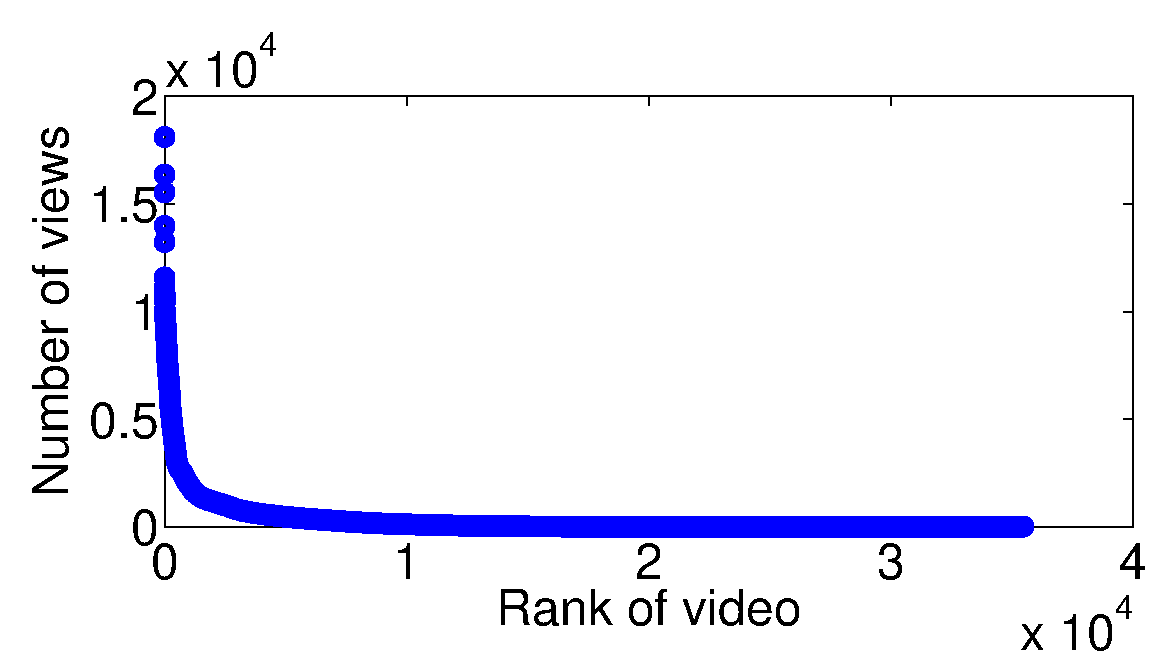
\includegraphics[width=.49\linewidth]{fig/video-freq.eps}
		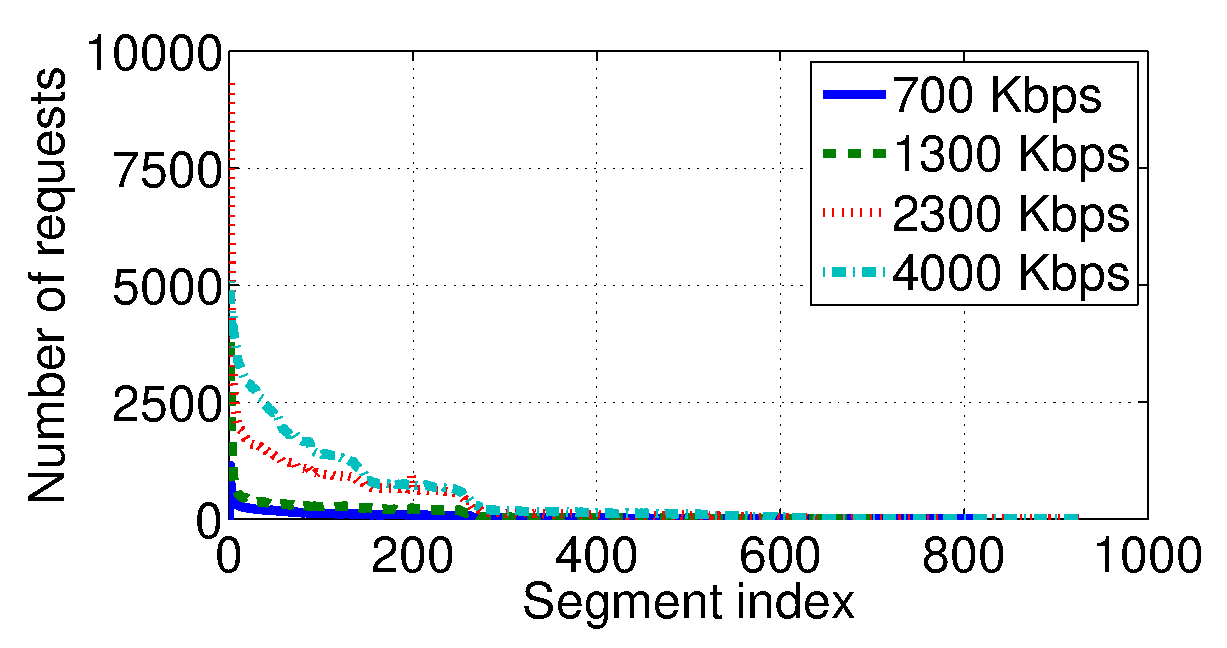
\includegraphics[width=.49\linewidth]{fig/sy-req-vs-seg.eps}
		%\item in WeiShi (UGC)\\
		%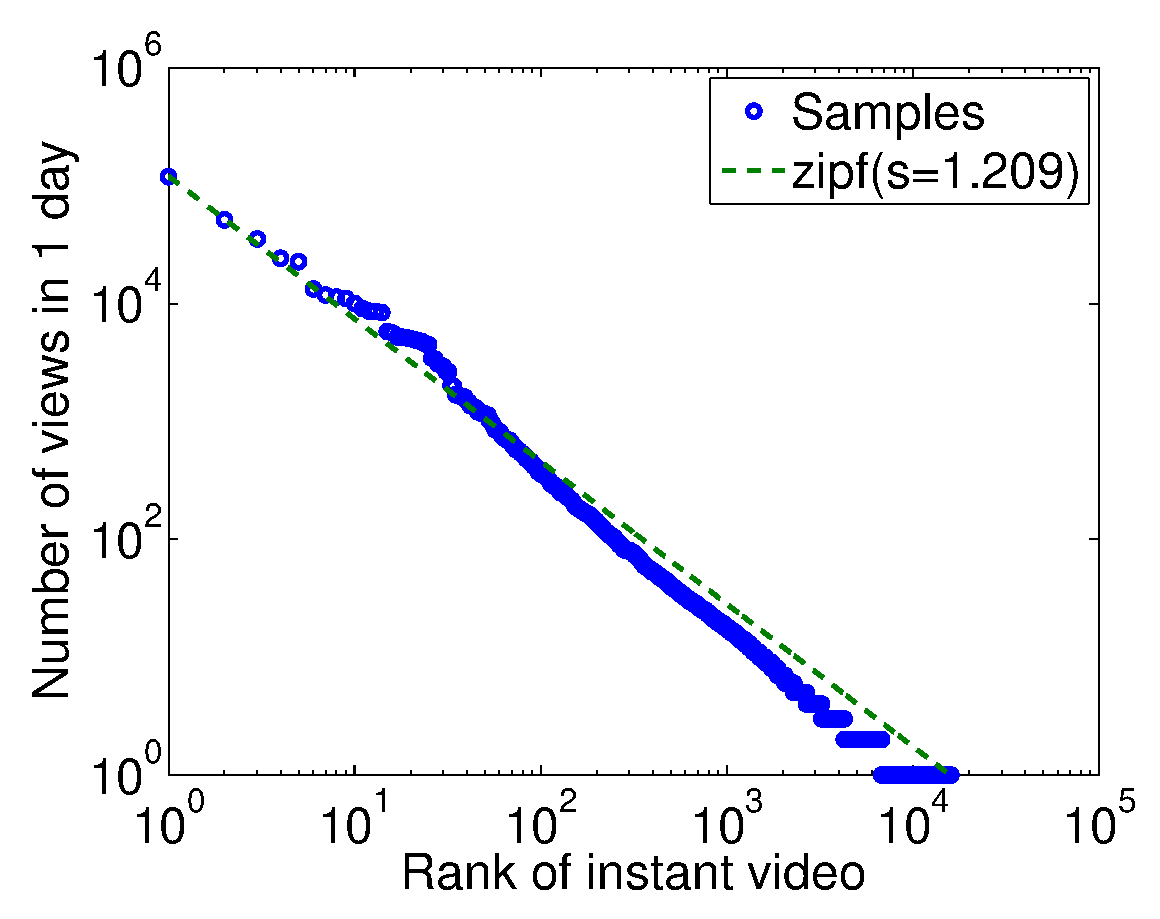
\includegraphics[width=.32\linewidth]{fig/video-popularity.eps}
		%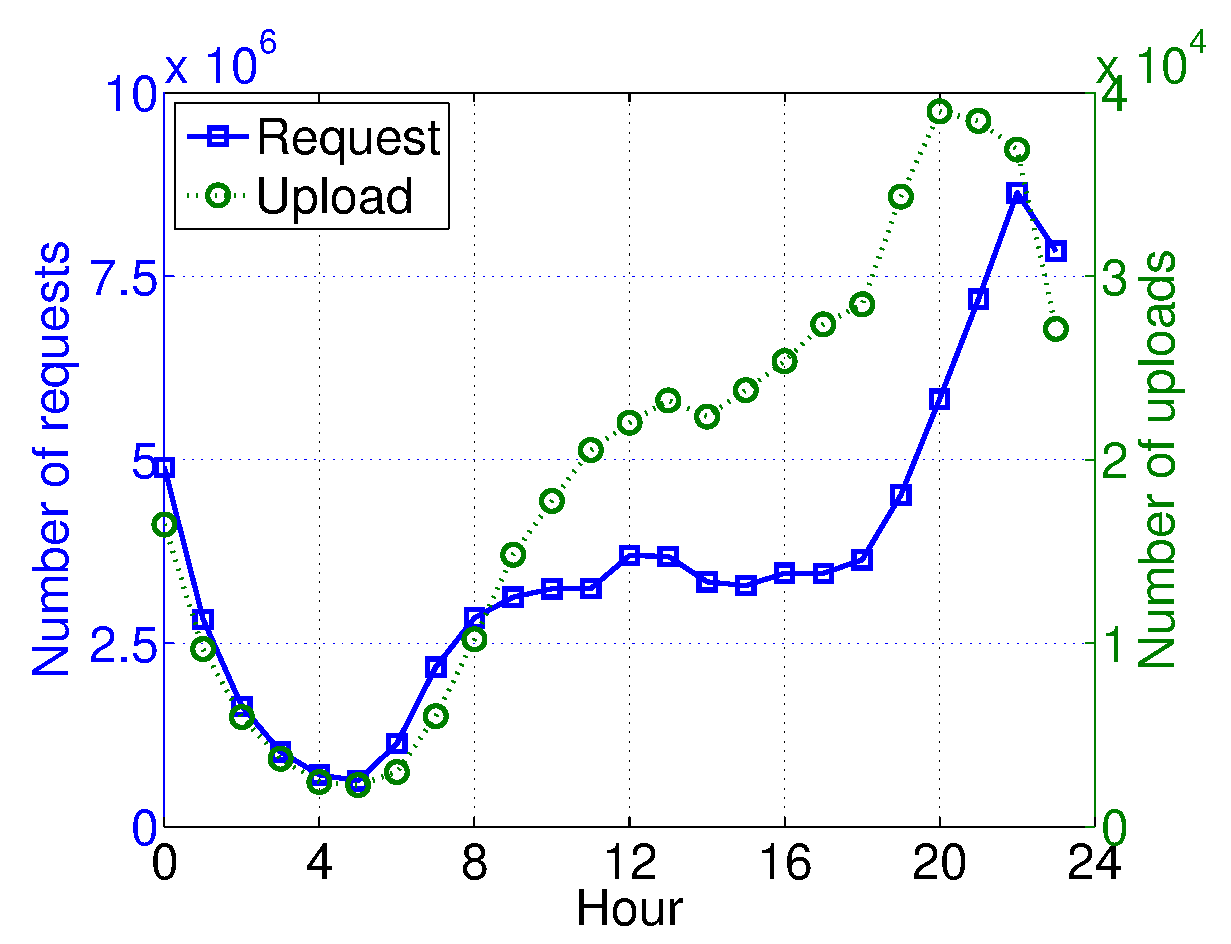
\includegraphics[width=.24\linewidth]{fig/request-upload-overtime.eps}
		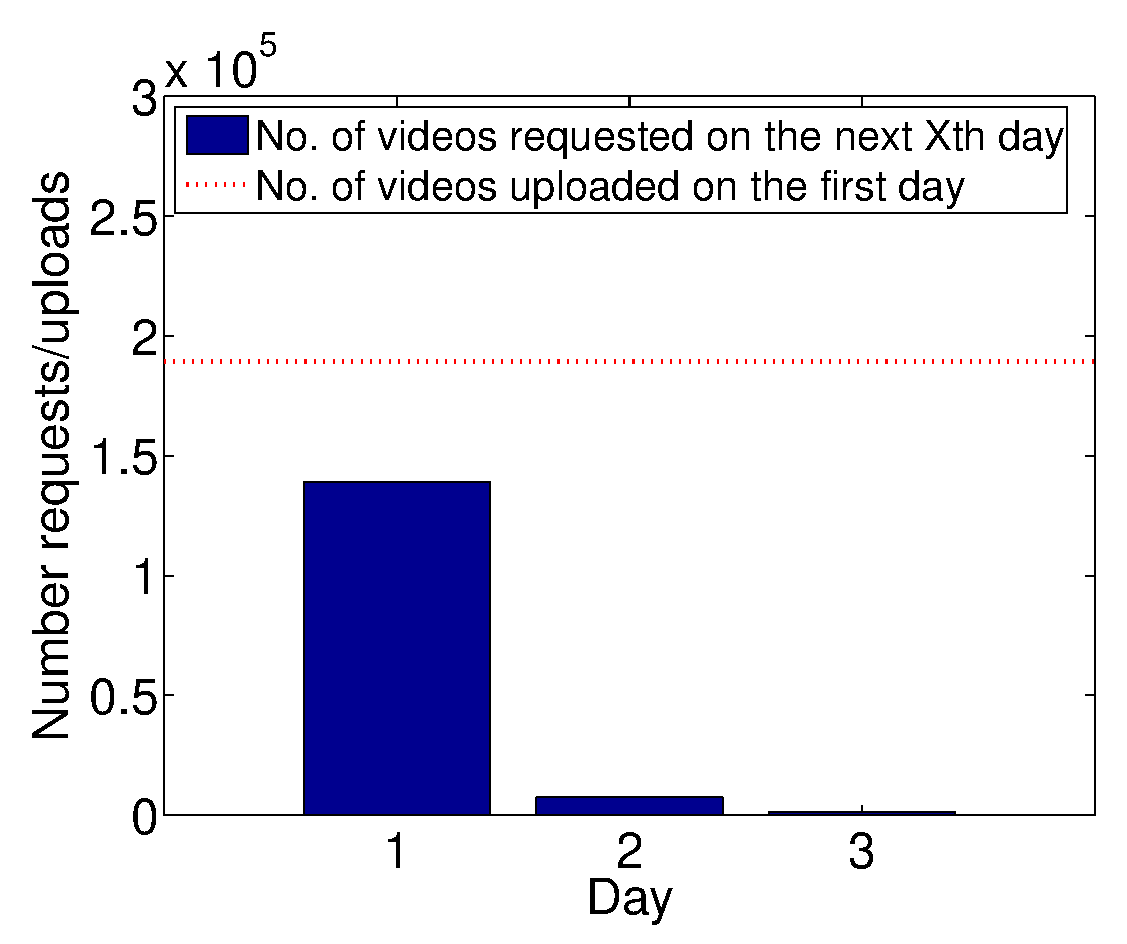
\includegraphics[width=.46\linewidth]{fig/view-in-3-days.eps}
		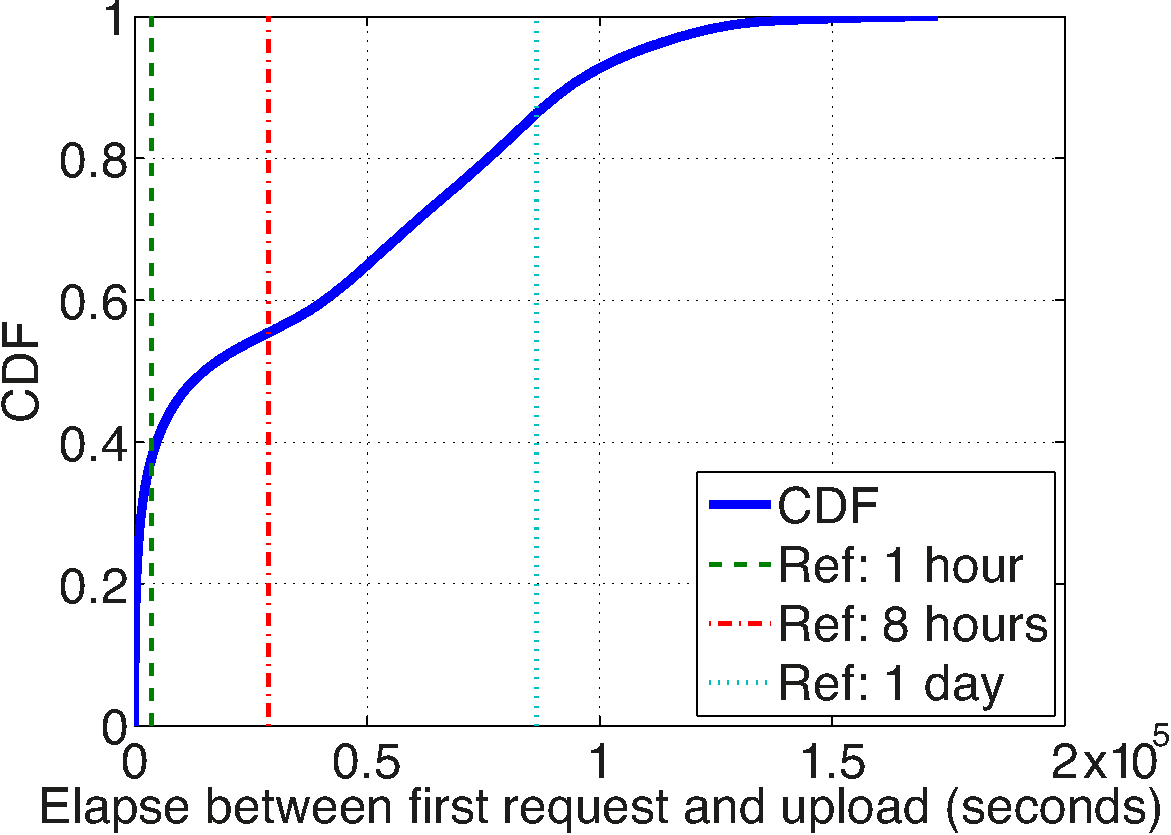
\includegraphics[width=.50\linewidth]{fig/updowntimediff.pdf}\\
	%\end{itemize}
	CDN Patterns (CPU load \& bandwidth)\\
	%\begin{itemize}
		%\item CPU load patterns\\
		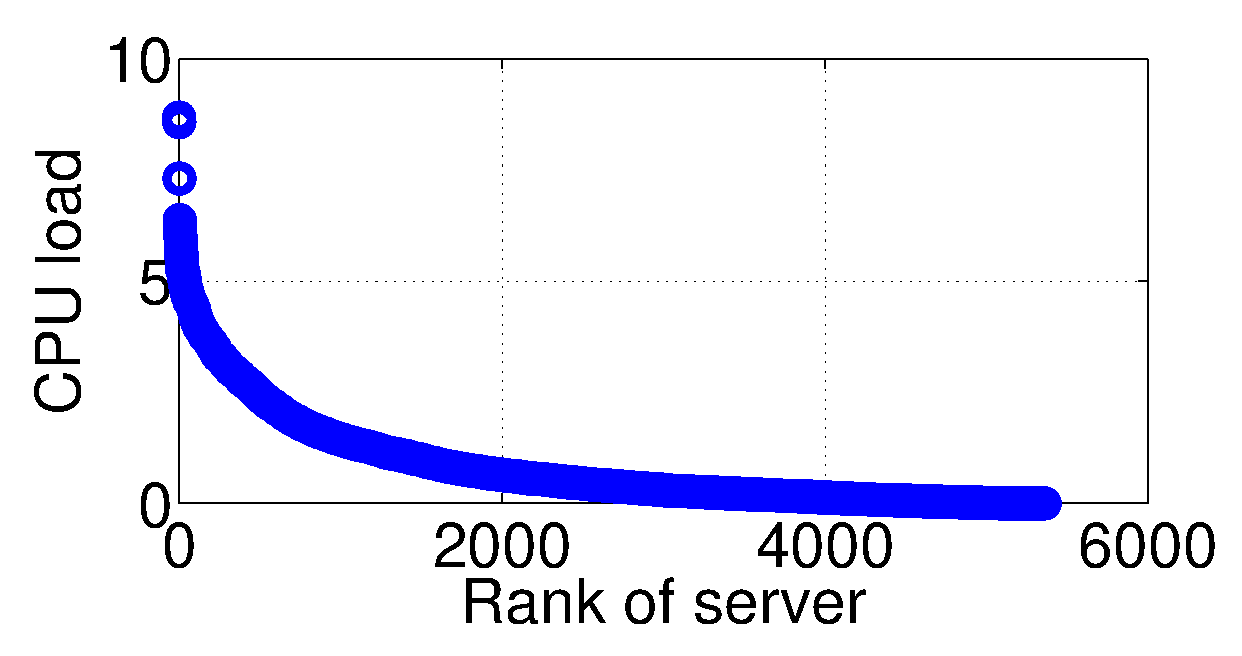
\includegraphics[width=0.48\linewidth]{fig/cpuload_vs_server.eps}
		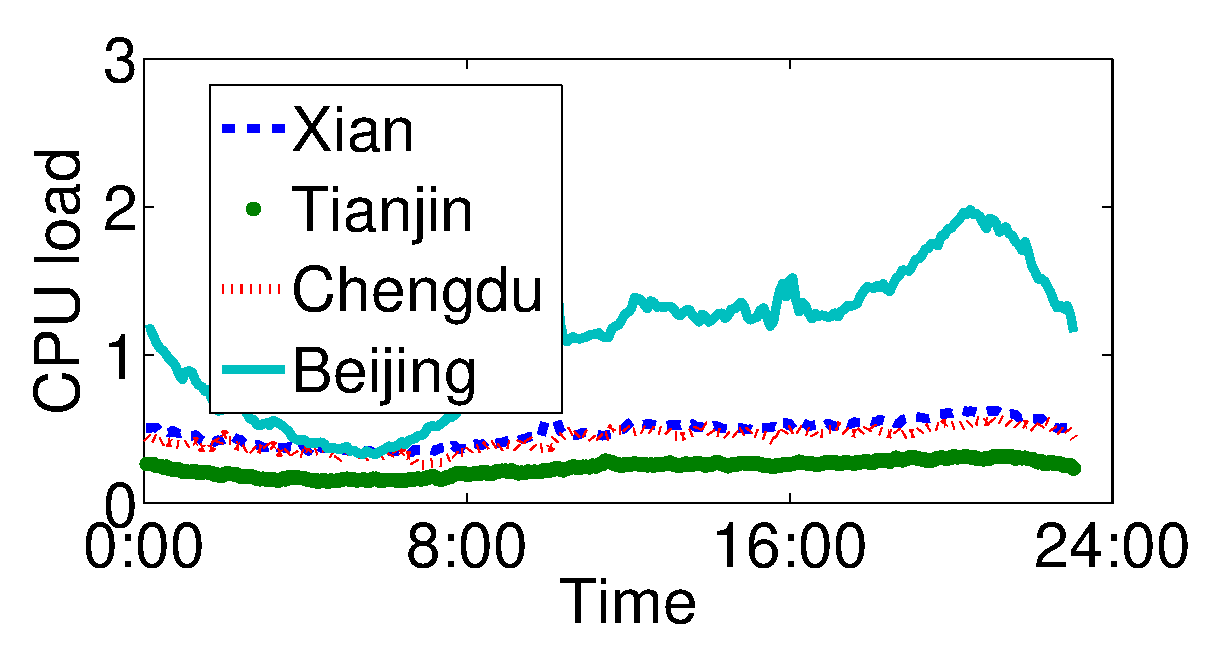
\includegraphics[width=0.48\linewidth]{fig/idc_cpuload_over_time.eps}
		%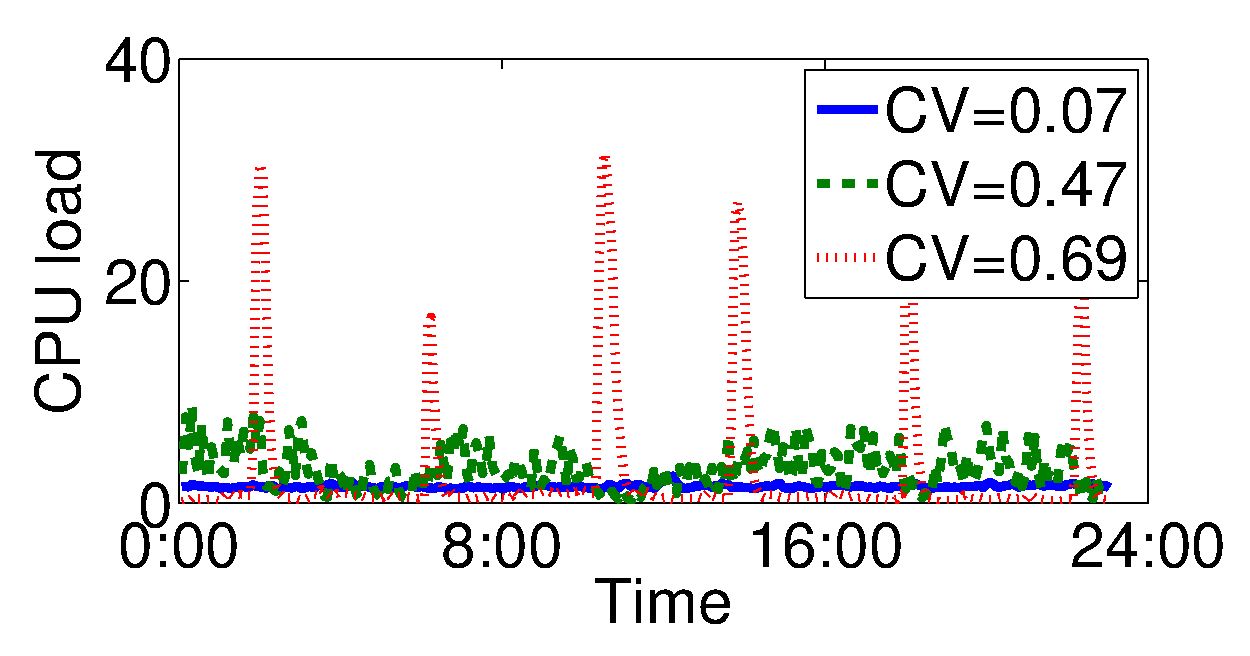
\includegraphics[width=0.32\linewidth]{fig/server_cpu_load_overtime.eps}
		%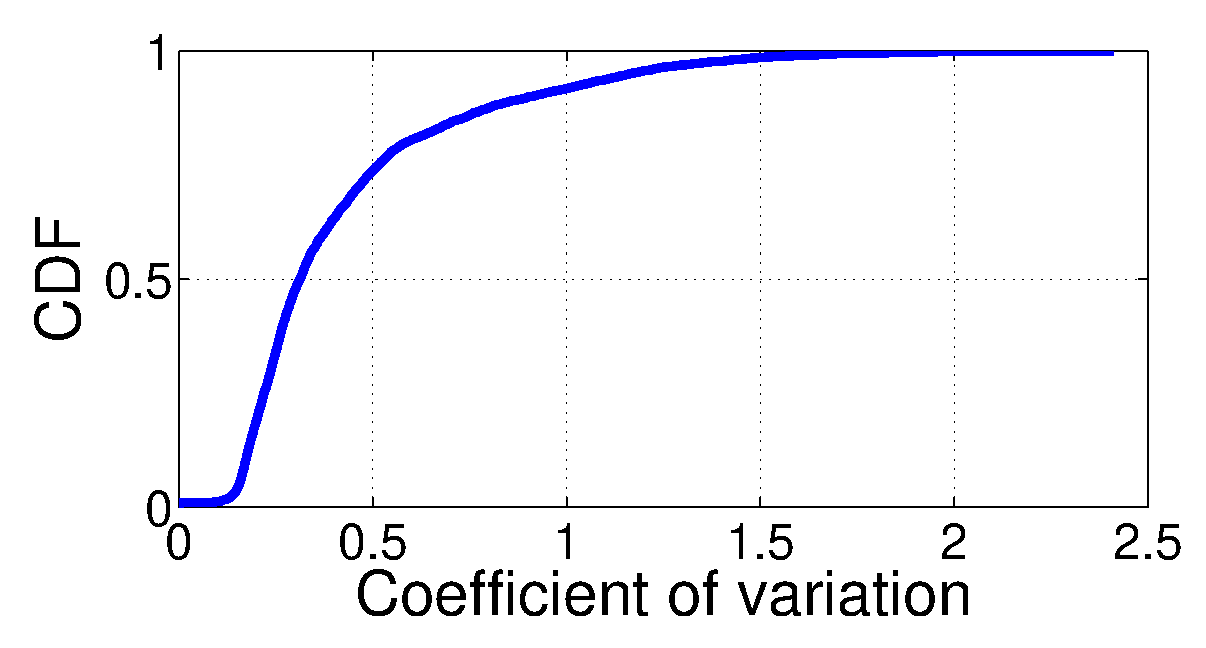
\includegraphics[width=0.24\linewidth]{fig/server_cv_cdf.eps}\\
		%\footnote{$CV = 1/24 \sum_{h=0}^{23} {\sqrt{E[(X_h - \bar{X_h})^2]}}/{\bar{X_h}}$, $X_h$: CPU load in $h$}
		%\item total bandwidth of a CDN region; CPU utilization of a server\\
		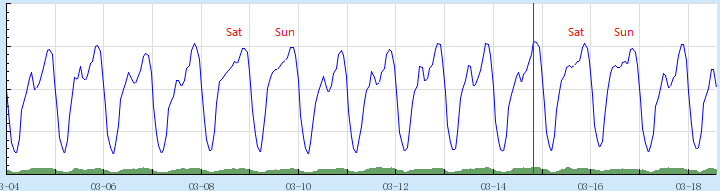
\includegraphics[width=0.65\linewidth]{fig/bandwidth.png}
		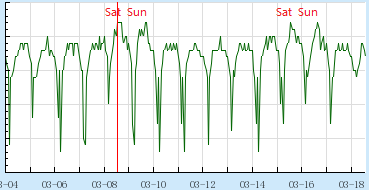
\includegraphics[width=0.34\linewidth]{fig/cpu_utilization.png}\\
		%\item bandwidth patterns\\
		%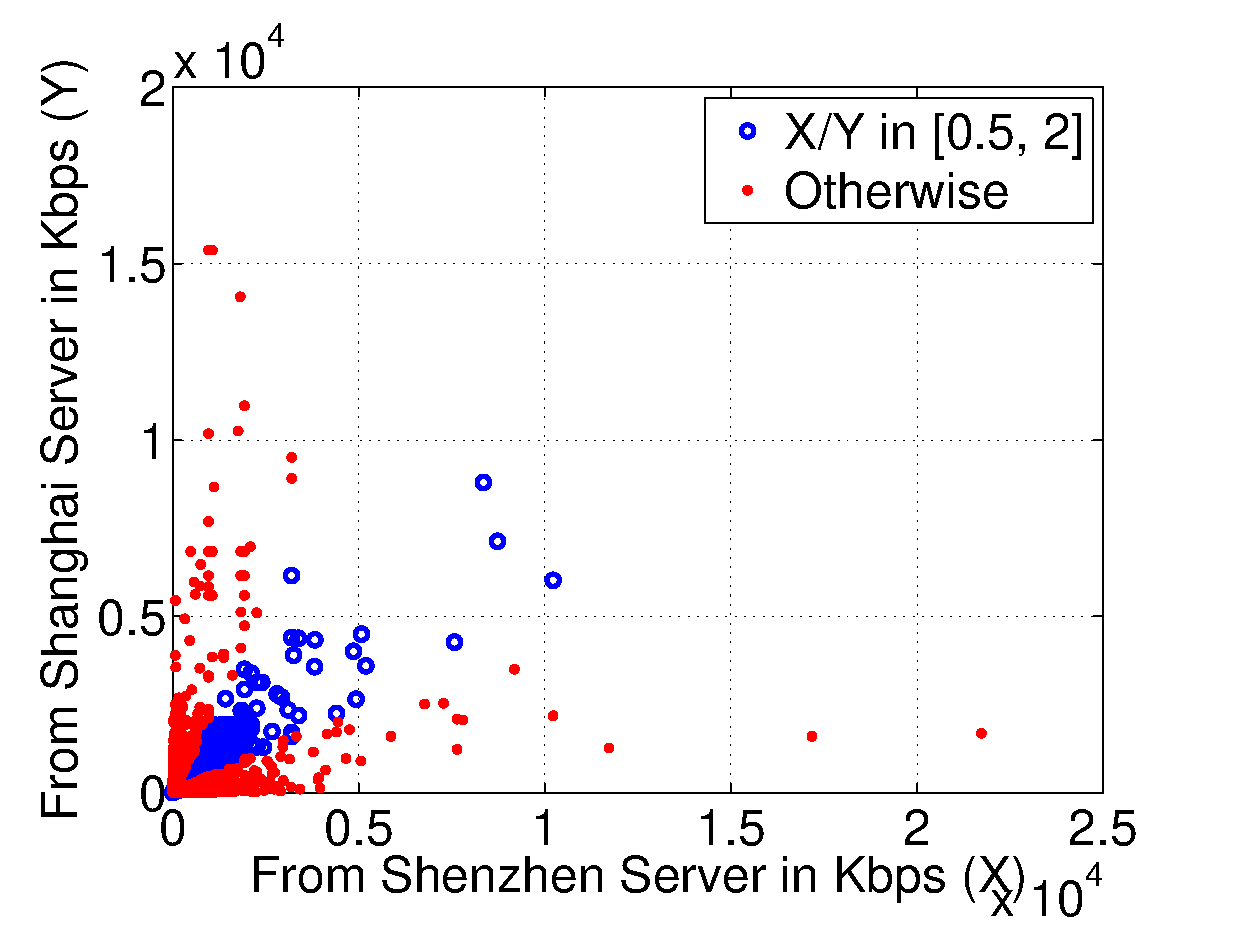
\includegraphics[width=0.24\linewidth]{fig/user-server-speed.eps}
		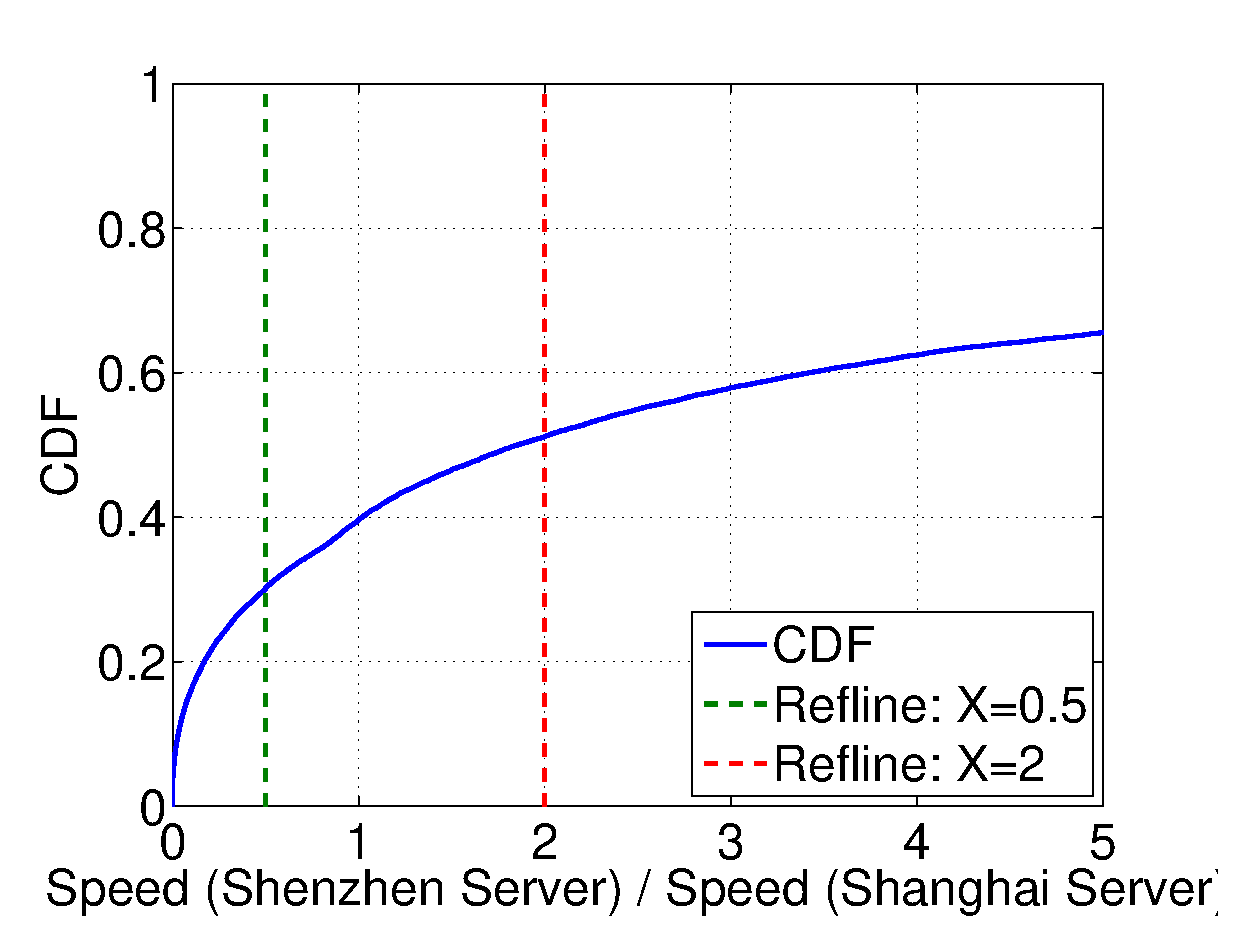
\includegraphics[width=0.44\linewidth]{fig/user-server-speed-ratio.eps}
		%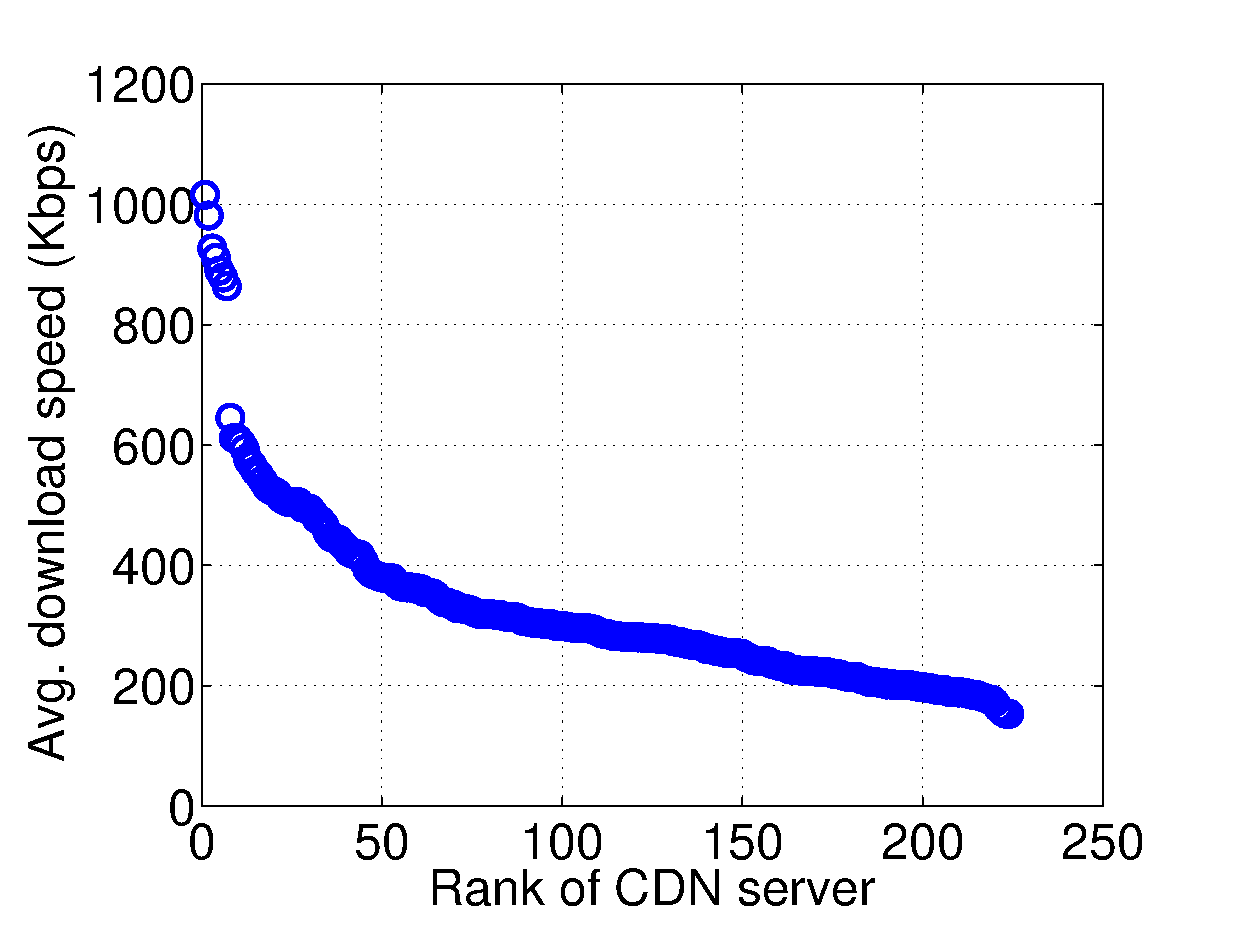
\includegraphics[width=0.23\linewidth]{fig/tencent_cdn_server_downloadspeed_20130504.eps}
		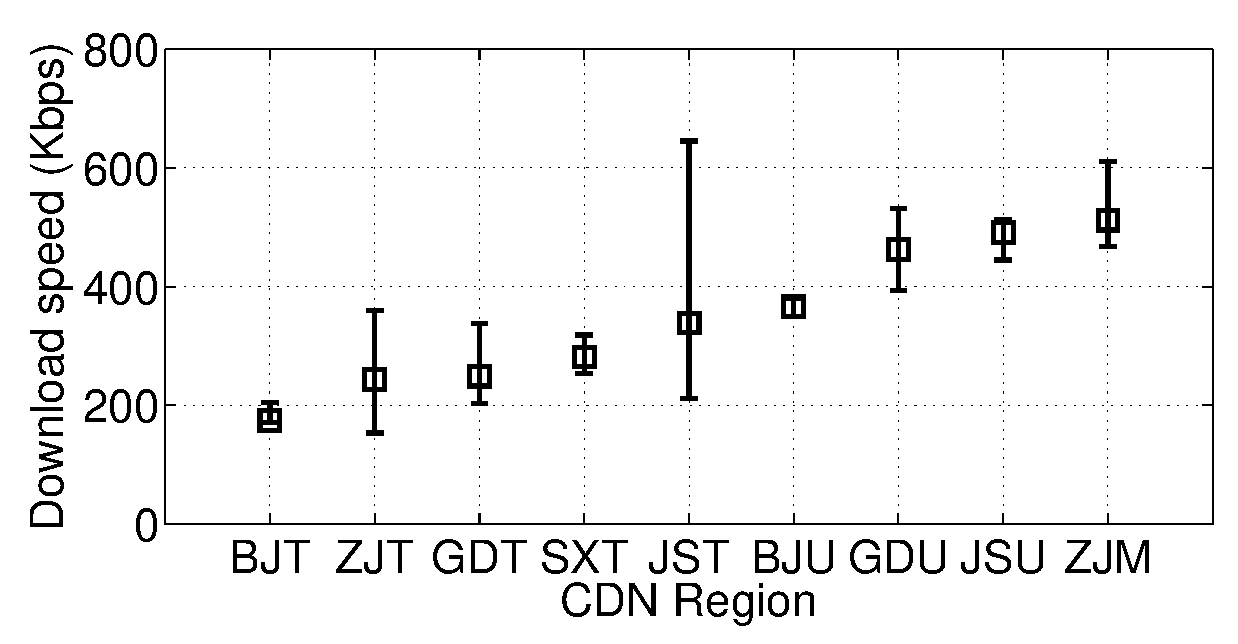
\includegraphics[width=0.55\linewidth]{fig/region-speed-distribution.eps}\\
	%\end{itemize}
	%\begin{itemize}
	%\end{itemize}
	Insights:\\
	%\begin{itemize}
		$\star \S$ No necessary to pre-transcode/store all\\
		%pre-transcoding every segment of all videos to an increasing number of versions is a huge waste of computing resource
		$\star \S$ Most backend servers in CDNs are predictably(stably) idle\\
		\indent Can be scheduled for transcoding?\\
		$\star \S$ users have preferences in CDN regions\\
		$\star \S$ regions have preferences in media versions
	%\end{itemize}
}
%%%%%%%%%%%%%%%%%%%%%%%%%%%%%%%%%%%%%%%%%%%%%%%%%%%%%%%%%%%%%%%%%%%%%%%%%%%%%%
\headerbox{Framework}{name=framework,span=1,column=1,above=bottom}{
\noindent
3 phases joint optimization\\
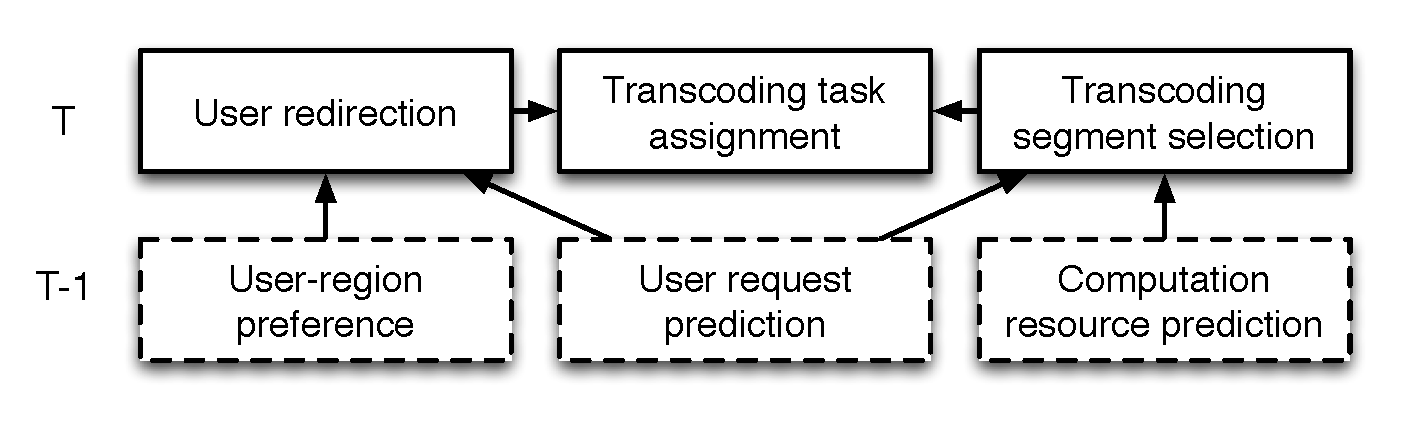
\includegraphics[width=1.0\linewidth]{fig/framework.eps}
}
%%%%%%%%%%%%%%%%%%%%%%%%%%%%%%%%%%%%%%%%%%%%%%%%%%%%%%%%%%%%%%%%%%%%%%%%%%%%%%
\headerbox{Methods}{name=methods,span=2,column=2}{
	%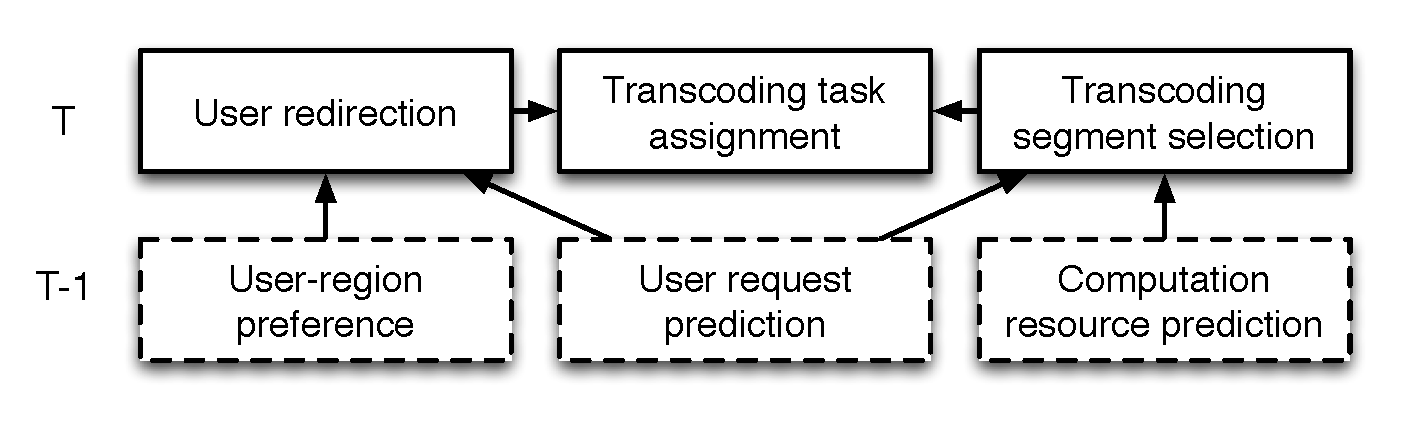
\includegraphics[width=0.4\linewidth]{fig/framework.eps}\\
	\noindent
	\emph{Girls} Chasing \emph{Boys}! (Stable Maching plus Linear Programming)
	\begin{center}
		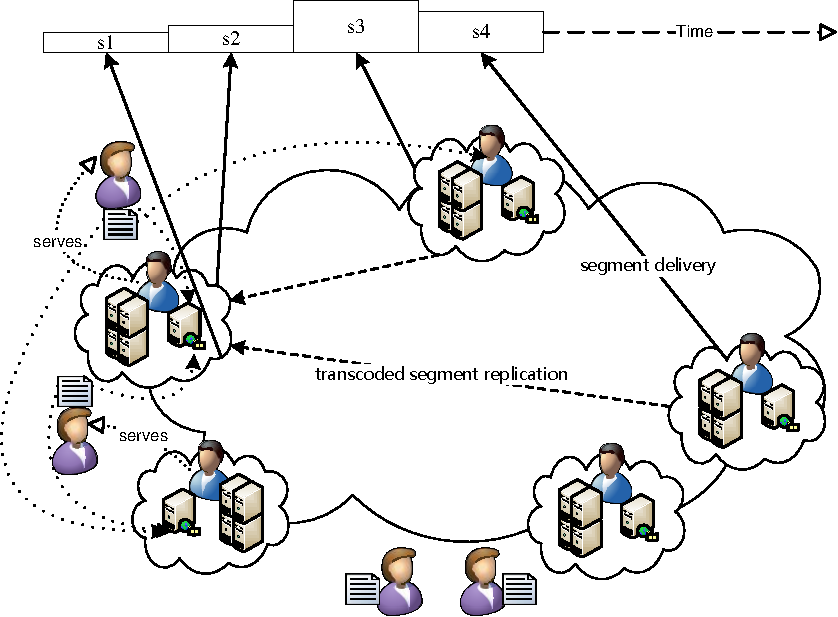
\includegraphics[width=0.73\linewidth]{fig/transcoding_delivery.pdf}
	\small{
		$
		\max_{\Redirect^{(T)}} \sum_{u \in \Users^{(T)}, r \in \CDNRegions} \USPref_{u,r} \Redirect^{(T)}_{u,r}; ~
		\label{eq:redirect}
		$
		$
		\max_{\TranscodeIndicator^{(T)}} \sum_{(s,v) \in \RequestingSeg^{(T)}} \TranscodeIndicator^{(T)}_{(s,v)} e_{(s,v)}^{(T)}; ~
		$
		$
		\min_{\Assign^{(T)}} \sum_{(s,v) \in \TranscodeSet^{(T)}} \sum_{r \in \CDNRegions} \Assign^{(T)}_{(s,v),r} \SegRepCost_{(s,v), r}
		$
	}
	\end{center}
}
%%%%%%%%%%%%%%%%%%%%%%%%%%%%%%%%%%%%%%%%%%%%%%%%%%%%%%%%%%%%%%%%%%%%%%%%%%%%%%
\headerbox{Resuls}{name=results,column=2,above=bottom}{
\noindent
%\begin{itemize}
	%\item Computing resource saved\\
		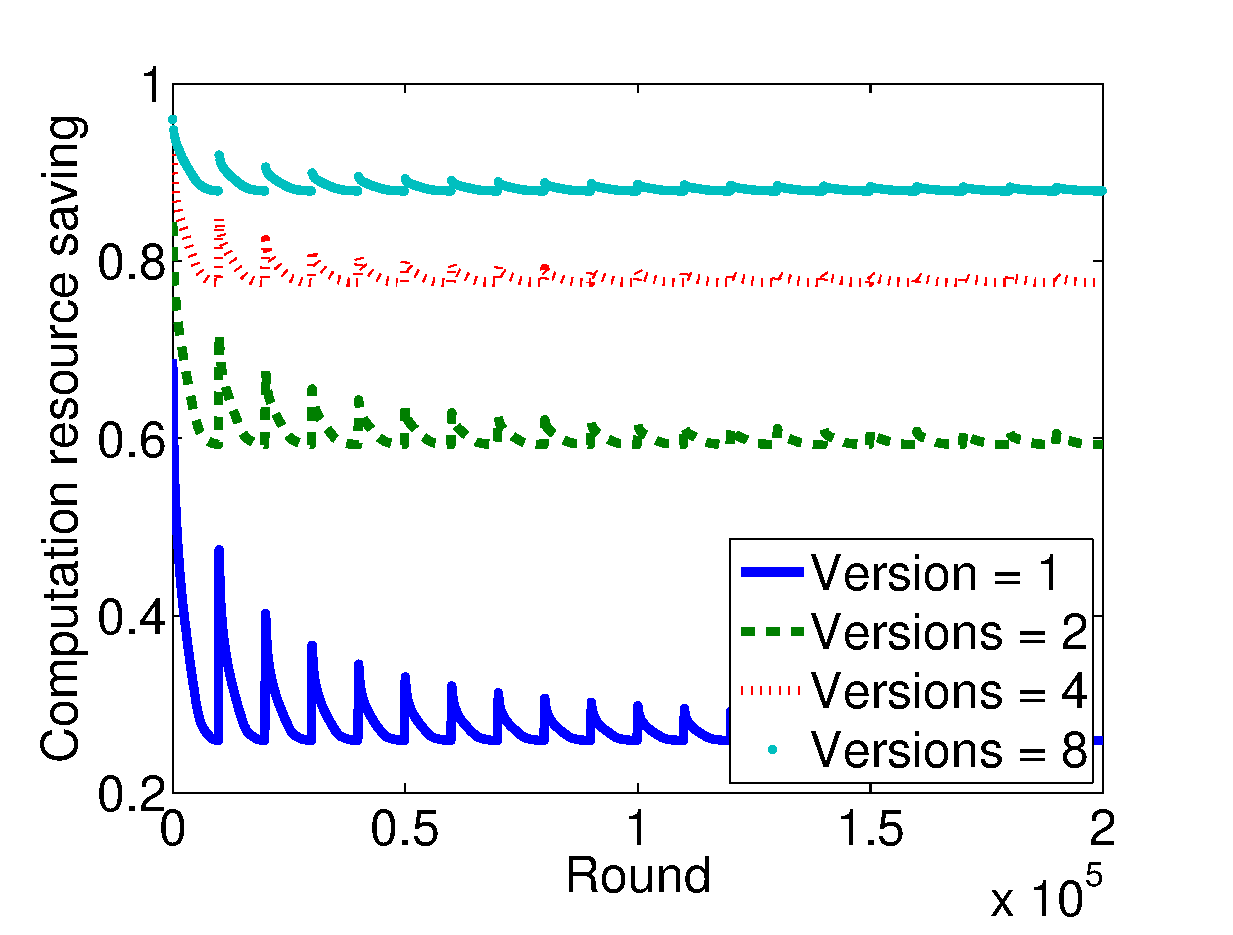
\includegraphics[width=0.48\linewidth]{fig/comp-saved-overtime-vs-ver-iter.eps}
		%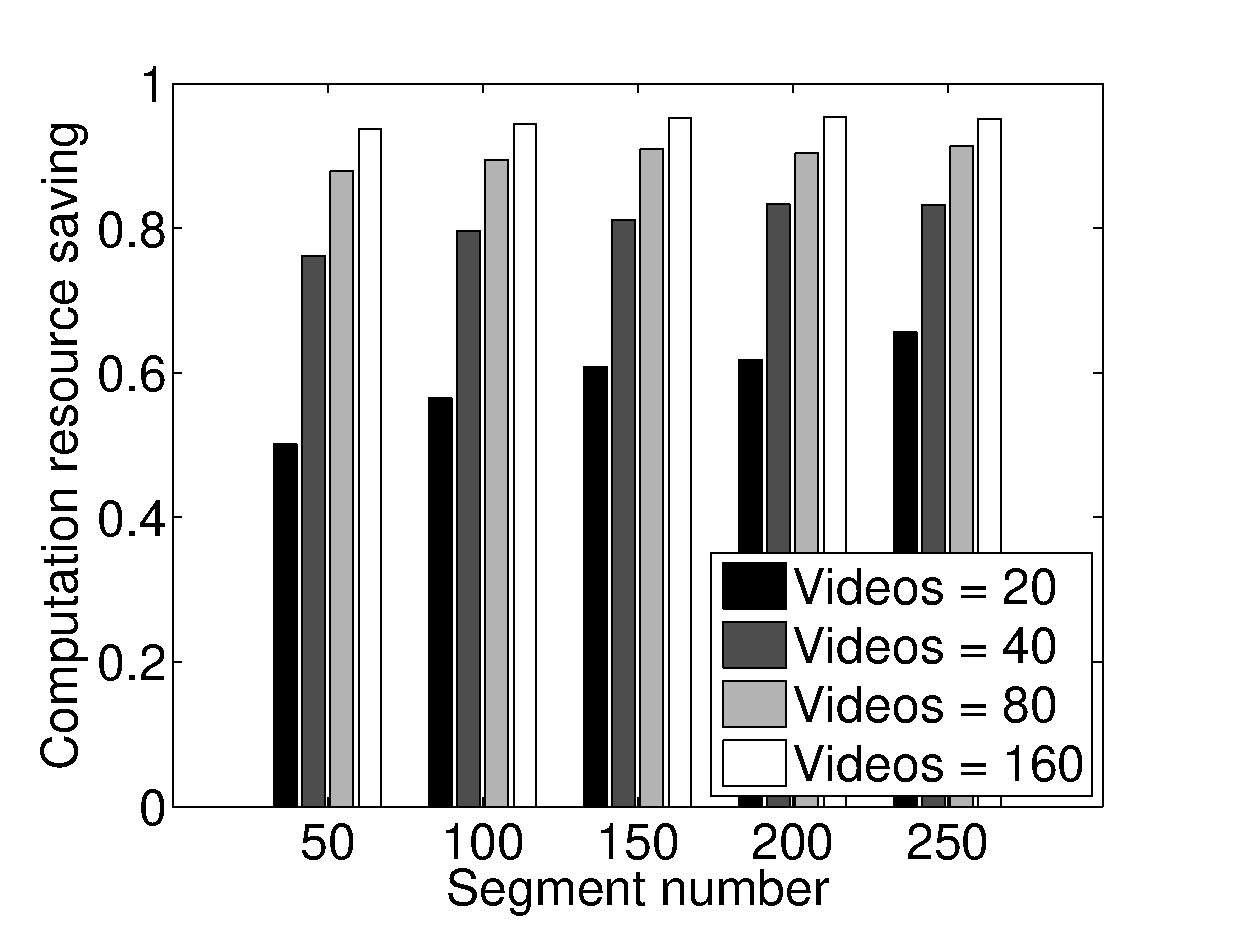
\includegraphics[width=0.44\linewidth]{fig/comp-saved-overtime-vs-vseg.eps}
	%\item Improvement of QoE\\
		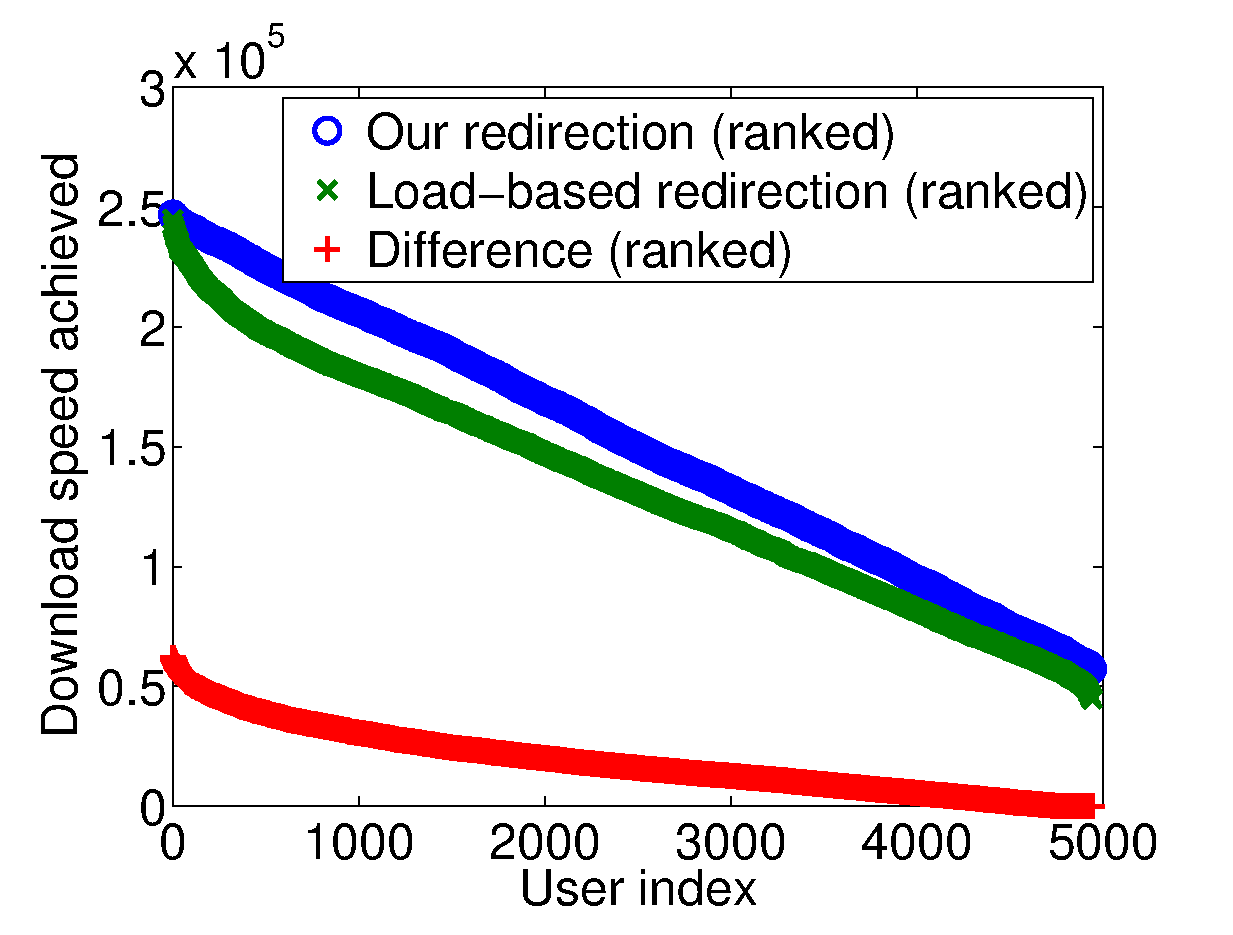
\includegraphics[width=0.48\linewidth]{fig/redirection-cmp.eps}
		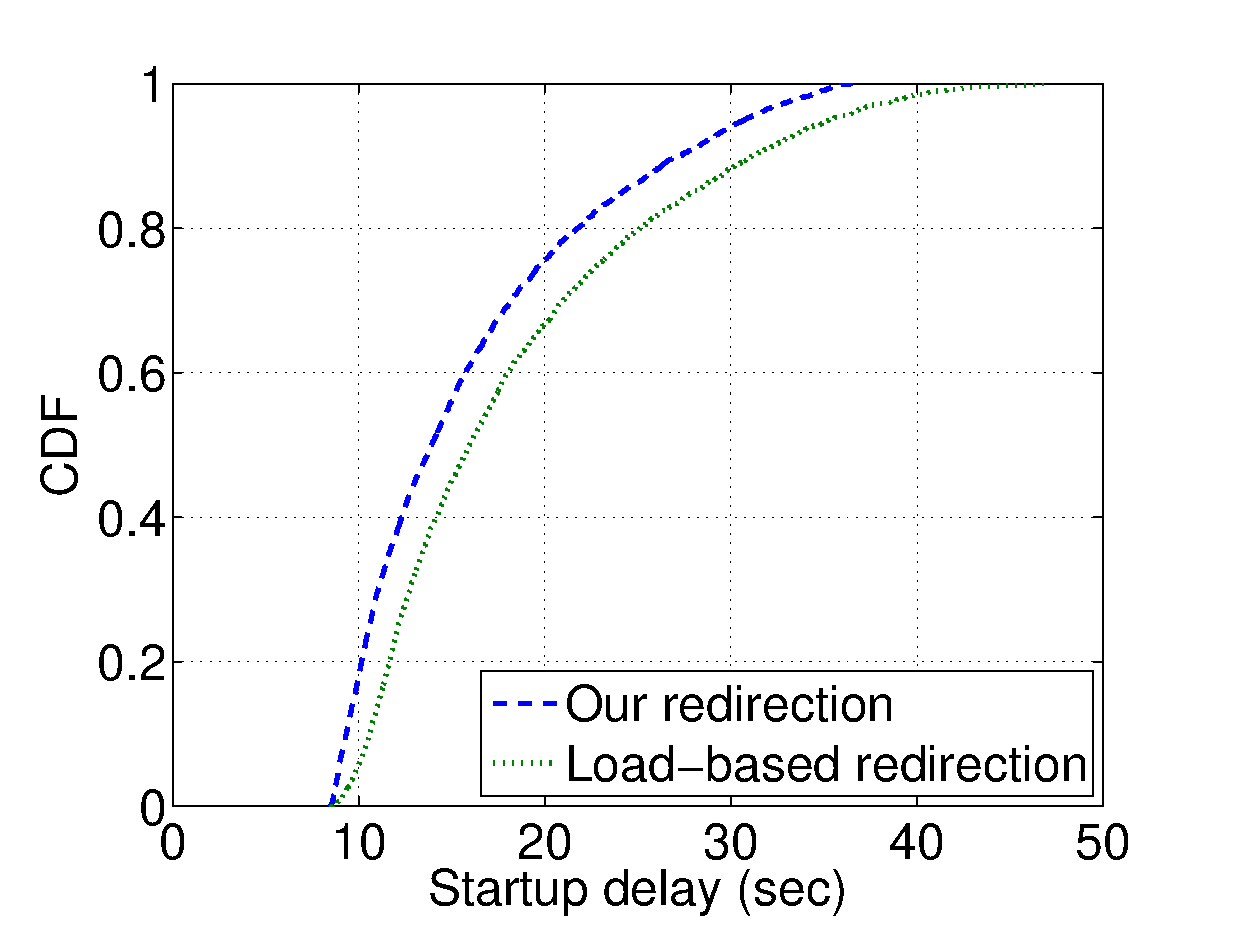
\includegraphics[width=0.48\linewidth]{fig/startup-delay.eps}
		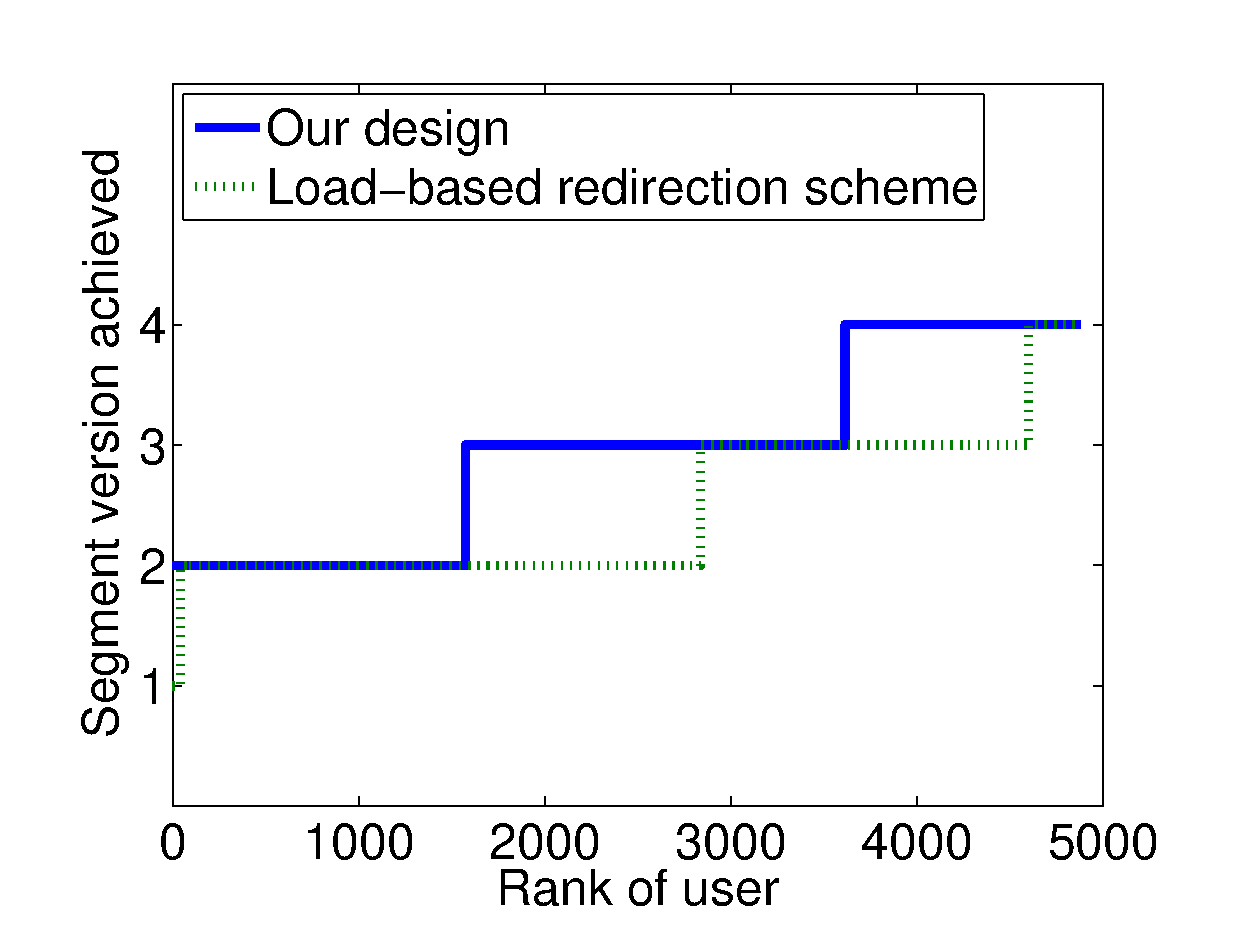
\includegraphics[width=0.48\linewidth]{fig/redirection-ver-cmp.eps}
	%\item Mismatch\\
		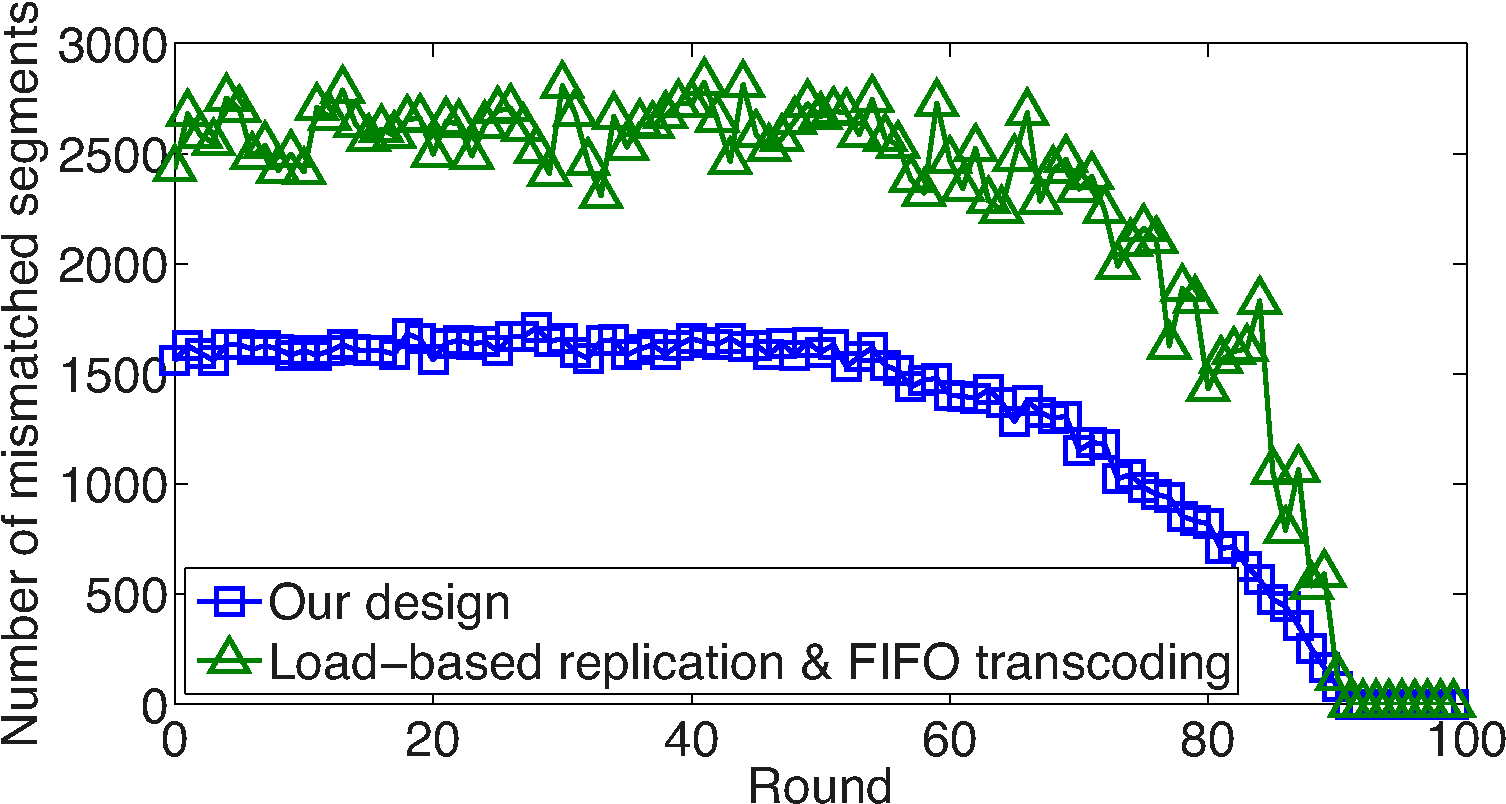
\includegraphics[width=0.55\linewidth]{fig/mismatch-overtime.pdf}
	%\item Replication Cost\\
		%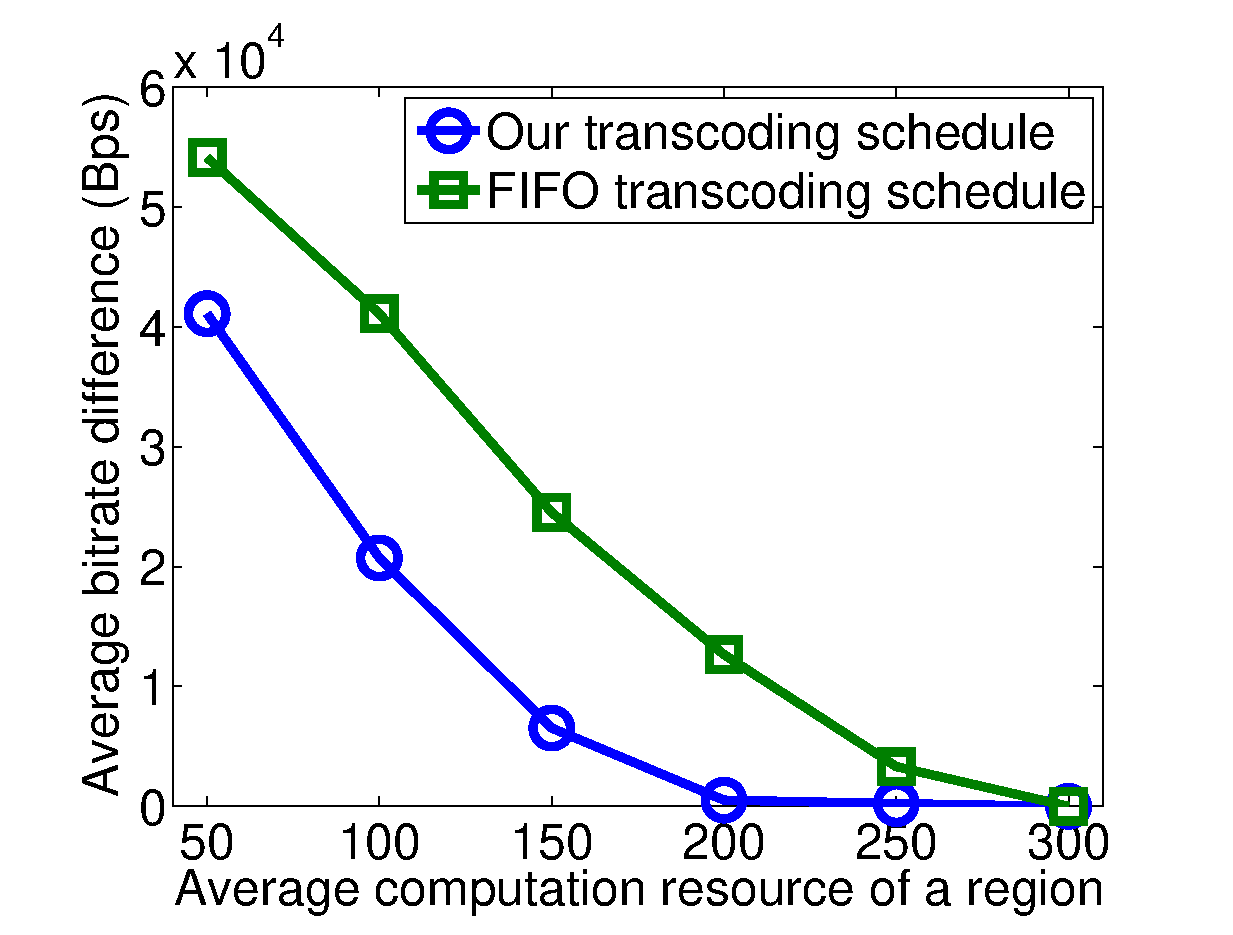
\includegraphics[width=0.32\linewidth]{fig/transcode-cmp-mismatchbit.eps}
		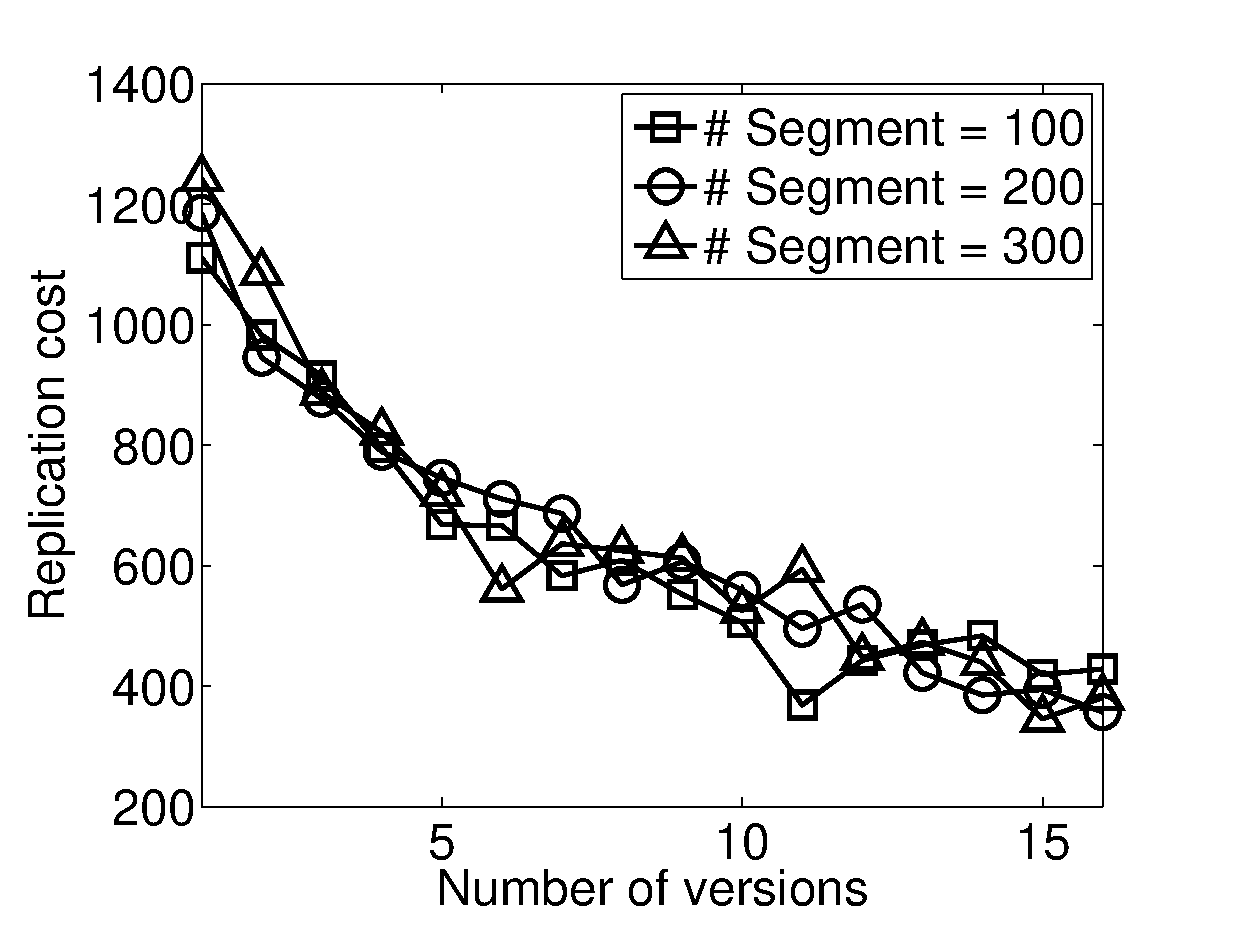
\includegraphics[width=0.41\linewidth]{fig/replication-cost-vs-version.eps}	
%\end{itemize}
}
%%%%%%%%%%%%%%%%%%%%%%%%%%%%%%%%%%%%%%%%%%%%%%%%%%%%%%%%%%%%%%%%%%%%%%%%%%%%%%
\headerbox{Hightlights}{name=highlights,column=3,below=methods,aligned=results}{
	\noindent
	\begin{itemize}
		\item $44.8\%$  users enjoy higher bitrate versions than the load-balanced redirection scheme
		\item $4.5$x users enjoy the highest possible bitrate
		\item Mismatch rate reduced by over $42.2\%$
		\item $\sim 80\%$ computing resource saved when the number of versions is 4.\\
		The higher the number is, the more resource our approach saves. 
	\end{itemize}
}
%%%%%%%%%%%%%%%%%%%%%%%%%%%%%%%%%%%%%%%%%%%%%%%%%%%%%%%%%%%%%%%%%%%%%%%%%%%%%%
\headerbox{Afterword}{name=afterword,column=3,above=bottom}{
\noindent 
Transcoding and delivery can, and should be considered \& done jointly.\\
$\S$ A joint work with THU, HKU, Tencent.\\
$\S$ Appeared in IEEE TMM 2015.\\
$\S$ In serving WeChat video clip, QZone video...
}

\end{poster}

\end{document}
